\begin{figure}
  \centering
  \hspace*{-0.15\textwidth}%
  \begin{subfigure}[t]{0.125\textwidth}
    \tikzstyle{legend-point}=[circle, inner sep=2pt]
    \definecolor{legend1}{HTML}{4c72b0}
    \definecolor{legend2}{HTML}{55a868}
    \definecolor{legend3}{HTML}{c44e52}
    \definecolor{legend4}{HTML}{8172b2}
    \definecolor{legend5}{HTML}{ccb974}
    
    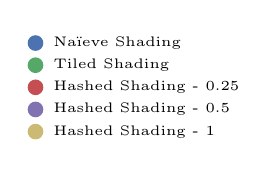
\begin{tikzpicture}
      \node (legend1) at (0.\textwidth, 0)
            [legend-point, fill={legend1}, label=right:{\tiny Na\"ieve Shading}] {};
      \node (legend2) at (0.\textwidth, -8pt)
            [legend-point, fill={legend2}, label=right:{\tiny Tiled Shading}] {};
      \node (legend3) at (0.\textwidth, -16pt)
            [legend-point, fill={legend3}, label=right:{\tiny Hashed Shading - 0.25}] {};
      \node (legend6) at (0.\textwidth, -24pt)
            [legend-point, fill={legend4}, label=right:{\tiny Hashed Shading - 0.5}] {};
      \node (legend7) at (0.\textwidth, -32pt)
            [legend-point, fill={legend5}, label=right:{\tiny Hashed Shading - 1}] {};
    \end{tikzpicture}
  \end{subfigure} %
  \begin{adjustbox}{minipage=0.4\textwidth, scale=0.6}
    \begin{subfigure}[b]{1.6\textwidth}
      \centering
      \def\svgwidth{\textwidth}
      \input{./img/raw/hs-compare-frames-exec/forward/frame_pipers-alley.pdf_tex}
      \caption{Piper's Alley}
      \vspace{4pt}
      \label{fig:hs-compare-frames:forward:alley}
    \end{subfigure}
  \end{adjustbox} \hspace{0.125\textwidth} %
  %
  \begin{adjustbox}{minipage=0.4\textwidth, scale=0.6}
    \begin{subfigure}[b]{1.6\textwidth}
      \centering
      \def\svgwidth{\textwidth}
      \input{./img/raw/hs-compare-frames-exec/forward/frame_ziggurat-city.pdf_tex}
      \caption{Ziggurat City}
      \label{fig:hs-compare-frames:forward:city}
    \end{subfigure}
  \end{adjustbox}
  \caption{\small The execution time per frame of Forward Shading.}
  \label{fig:hs-compare-frames:forward}
  % ----------------------------------------------------------------------------------------------------
  \hspace*{-0.15\textwidth}%
  \begin{subfigure}[t]{0.125\textwidth}
    \tikzstyle{legend-point}=[circle, inner sep=2pt]
    \definecolor{legend1}{HTML}{4c72b0}
    \definecolor{legend2}{HTML}{55a868}
    \definecolor{legend3}{HTML}{c44e52}
    \definecolor{legend4}{HTML}{8172b2}
    \definecolor{legend5}{HTML}{ccb974}
    
    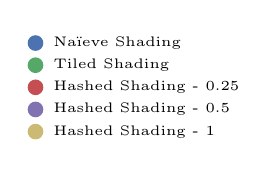
\begin{tikzpicture}
      \node (legend1) at (0.\textwidth, 0)
            [legend-point, fill={legend1}, label=right:{\tiny Na\"ieve Shading}] {};
      \node (legend2) at (0.\textwidth, -8pt)
            [legend-point, fill={legend2}, label=right:{\tiny Tiled Shading}] {};
      \node (legend3) at (0.\textwidth, -16pt)
            [legend-point, fill={legend3}, label=right:{\tiny Hashed Shading - 0.25}] {};
      \node (legend6) at (0.\textwidth, -24pt)
            [legend-point, fill={legend4}, label=right:{\tiny Hashed Shading - 0.5}] {};
      \node (legend7) at (0.\textwidth, -32pt)
            [legend-point, fill={legend5}, label=right:{\tiny Hashed Shading - 1}] {};
    \end{tikzpicture}
  \end{subfigure} %
  \begin{adjustbox}{minipage=0.4\textwidth, scale=0.6}
    \begin{subfigure}[b]{1.6\textwidth}
      \centering
      \def\svgwidth{\textwidth}
      \input{./img/raw/hs-compare-frames-exec/deferred/frame_pipers-alley.pdf_tex}
      \caption{Piper's Alley}
      \vspace{4pt}
      \label{fig:hs-compare-frames:deferred:alley}
    \end{subfigure}
  \end{adjustbox}  \hspace{0.125\textwidth} %
  %
  \begin{adjustbox}{minipage=0.4\textwidth, scale=0.6}
    \begin{subfigure}[b]{1.6\textwidth}
      \centering
      \def\svgwidth{\textwidth}
      \input{./img/raw/hs-compare-frames-exec/deferred/frame_ziggurat-city.pdf_tex}
      \caption{Ziggurat City}
      \label{fig:hs-compare-frames:deferred:city}
    \end{subfigure}
  \end{adjustbox}
  \caption{\small The execution time per frame of Deferred Shading.}
  \label{fig:hs-compare-frames:deferred}

  % ----------------------------------------------------------------------------------------------------
  \hspace*{-0.15\textwidth}%
  \begin{subfigure}[t]{0.125\textwidth}
    \tikzstyle{legend-point}=[circle, inner sep=2pt]
    \definecolor{legend1}{HTML}{4c72b0}
    \definecolor{legend2}{HTML}{55a868}
    \definecolor{legend3}{HTML}{c44e52}
    \definecolor{legend4}{HTML}{8172b2}
    \definecolor{legend5}{HTML}{ccb974}
    \definecolor{legend5}{HTML}{ccb974}
    \definecolor{legend6}{HTML}{64b5cd}
    
    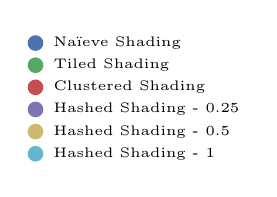
\begin{tikzpicture}
      \node (legend1) at (0.\textwidth, 0)
            [legend-point, fill={legend1}, label=right:{\tiny Na\"ieve Shading}] {};
      \node (legend2) at (0.\textwidth, -8pt)
            [legend-point, fill={legend2}, label=right:{\tiny Tiled Shading}] {};
      \node (legend2) at (0.\textwidth, -16pt)
            [legend-point, fill={legend3}, label=right:{\tiny Clustered Shading}] {};
      \node (legend3) at (0.\textwidth, -24pt)
            [legend-point, fill={legend4}, label=right:{\tiny Hashed Shading - 0.25}] {};
      \node (legend6) at (0.\textwidth, -32pt)
            [legend-point, fill={legend5}, label=right:{\tiny Hashed Shading - 0.5}] {};
      \node (legend7) at (0.\textwidth, -40pt)
            [legend-point, fill={legend6}, label=right:{\tiny Hashed Shading - 1}] {};
    \end{tikzpicture}
  \end{subfigure} %
  \begin{adjustbox}{minipage=0.4\textwidth, scale=0.6}
    \begin{subfigure}[b]{1.6\textwidth}
      \centering
      \def\svgwidth{\textwidth}
      \input{./img/raw/hs-compare-frames-lc/lc_pipers-alley.pdf_tex}
      \caption{Pipers Alley}
      \vspace{4pt}
      \label{fig:hs-compare-frames:lc:alley}
    \end{subfigure}
  \end{adjustbox} \hspace{0.125\textwidth} %\\
  %
  \begin{adjustbox}{minipage=0.4\textwidth, scale=0.6}
    \begin{subfigure}[b]{1.6\textwidth}
      \centering
      \def\svgwidth{\textwidth}
      \input{./img/raw/hs-compare-frames-lc/lc_ziggurat-city.pdf_tex}
      \caption{Ziggurat stad}
      \label{fig:hs-compare-frames:lc:city}
    \end{subfigure}
  \end{adjustbox}
  \caption{\small The number of light calculations per frame of Deferred Shading.}
  \label{fig:hs-compare-frames:lc}
  % ----------------------------------------------------------------------------------------------------
  \hspace*{-0.15\textwidth}%
  \begin{subfigure}[t]{0.125\textwidth}
    \tikzstyle{legend-point}=[circle, inner sep=2pt]
    \definecolor{legend1}{HTML}{4c72b0}
    \definecolor{legend2}{HTML}{55a868}
    \definecolor{legend3}{HTML}{c44e52}
    \definecolor{legend4}{HTML}{8172b2}
    \definecolor{legend5}{HTML}{ccb974}
    
    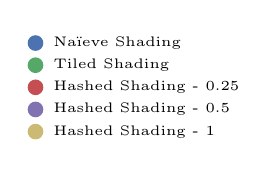
\begin{tikzpicture}
      \node (legend1) at (0.\textwidth, 0)
            [legend-point, fill={legend1}, label=right:{\tiny Na\"ieve Shading}] {};
      \node (legend2) at (0.\textwidth, -8pt)
            [legend-point, fill={legend2}, label=right:{\tiny Tiled Shading}] {};
      \node (legend3) at (0.\textwidth, -16pt)
            [legend-point, fill={legend3}, label=right:{\tiny Hashed Shading - 0.25}] {};
      \node (legend6) at (0.\textwidth, -24pt)
            [legend-point, fill={legend4}, label=right:{\tiny Hashed Shading - 0.5}] {};
      \node (legend7) at (0.\textwidth, -32pt)
            [legend-point, fill={legend5}, label=right:{\tiny Hashed Shading - 1}] {};
    \end{tikzpicture}
  \end{subfigure} %
  \begin{adjustbox}{minipage=0.4\textwidth, scale=0.6}
    \begin{subfigure}[b]{1.6\textwidth}
      \centering
      \def\svgwidth{\textwidth}
      \input{./img/raw/hs-compare-lights-exec/forward/lights_pipers-alley.pdf_tex}
      \caption{Piper's Alley}
      \vspace{4pt}
      \label{fig:hs-compare-lights:forward:alley}
    \end{subfigure}
  \end{adjustbox}  \hspace{0.125\textwidth} %
  %
  \begin{adjustbox}{minipage=0.4\textwidth, scale=0.6}
    \begin{subfigure}[b]{1.6\textwidth}
      \centering
      \def\svgwidth{\textwidth}
      \input{./img/raw/hs-compare-lights-exec/forward/lights_ziggurat-city.pdf_tex}
      \caption{Ziggurat City}
      \label{fig:hs-compare-lights:forward:city}
    \end{subfigure}
  \end{adjustbox}
  \caption{\small The execution time per frame as function of the number of lights for Forward Shading.}
  \label{fig:hs-compare-lights:forward}
\end{figure}

